\newSec[Regelerarten]{Arten von Reglergliedern}{2}

In diesem Kapitel sollen grundlegende Bausteine der Regelungtechnik beschrieben werden. Diesbezüglich erhebt dieses Kapitel keinen Anspruch auf Vollständigkeit. Auf eine detallierte Beschreibung, welche \ua\ das Zeitverhalten betrachten, soll hier außen vor gelassen werden.
Als weitere Einschränkung soll sich die Betrachtung der Bausteine ausschließlich auf zeitdiskrete Systeme (vgl. \refCap{zeitdiskrete Systeme}) beziehen.


\newSec[ControlP]{P-Glied}{3}
Die Abkürzung \texttt{P} in der Bezeichnung \textit{P-Glied} steht für \textit{proportional}. Hierbei wird eine die Eingangsgröße um einen Faktor $k_P$ verstärkt.
\missing[Elektrotechnik oder sehr einfacher Regler]
\missing[dauerhafte Regelabweichung.]

\begin{equ}[!ht]
\begin{equation}
y_k = k_P * x_k
\end{equation}
\caption{Übertragungsfunktion des P-Glieds}
\end{equ}


\begin{figure}[ht!]
\vspace{0.25cm}
\begin{center}
\fbox{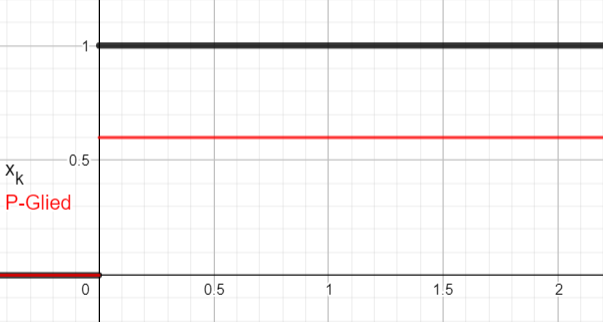
\includegraphics[width=8cm]{Pictures/StepP.png}}
\caption{Sprungantwort eines P-Glieds}
\label{fig:StepP}
\end{center}

\vspace{0.25cm}
\refImgShort{fig:StepPID} zeigt charakteristischen Sprungantwort des \textit{P-Glieds}. Hier wurde der Parameter $k_P$ mit dem Wert 0,6 gewählt, um die Sichtbarkeit in der Abbildung zu erhöhen.
\end{figure}

\missing[\cite{RT1} Seite 220]




\newSec[ControlI]{I-Gield}{3}
Wie sich aus dem Namen des \textit{Integral-Glieds} ableiten lässt, bildet dieser Baustein ein Integral über dem Eingangssignal.
Hierdurch können physikalische Umrechnungen oder Prozesse abgebildet werden. Als Beispiele kann an dieser Stelle der Füllstand eines Tanks oder die Ermittlung einer Geschwindigkeit aus Beschleunigungsdaten genannt werden.

\begin{equ}[!ht]
\begin{equation}
y_k = y_{k-1} + k_I * x_k*{\Delta t}
\end{equation}
\caption{Übertragungsfunktion des I-Glieds}
\end{equ}


\begin{figure}[ht!]
\vspace{0.25cm}
\begin{center}
\fbox{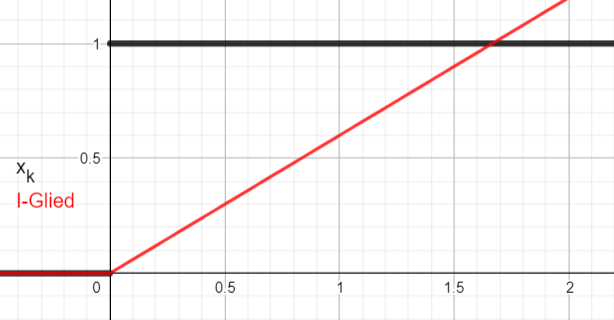
\includegraphics[width=8cm]{Pictures/StepI.png}}
\caption{Sprungantwort eines I-Glieds}
\label{fig:StepI}
\end{center}

\vspace{0.25cm}
\end{figure}






\newSec[ControlD]{D-Gield}{3}
In der betrachteten Literatur spielen D-Glieder keine signifikante Rolle. \compB{RT1}{SV1}
Dennoch sollen sie hier als Grundlage für \textit{PID}-Glieder beschrieben werden.

Bei einem \textit{D-Glied} handelt es sich um ein differentielles Glied. Somit lässt sich hiermit die Veränderung des Eingangssignals ermitteln.\comp{ContrD}\missing[Diese Quelle iO?]

Das Ausgangssignal des \textit{D-Glieds} kann durch folgende Formel berechnet werden, welche sich aus der Diskretisierung der Differenztationsfunktion ergibt.

\begin{equ}[!ht]
\begin{equation}
y_k = k_D * \frac{x_k - x_{k-1}}{\Delta t}
\end{equation}
\caption{Übertragungsfunktion des I-Glieds}
\end{equ}


\begin{figure}[ht!]
\vspace{0.25cm}
\begin{center}
\fbox{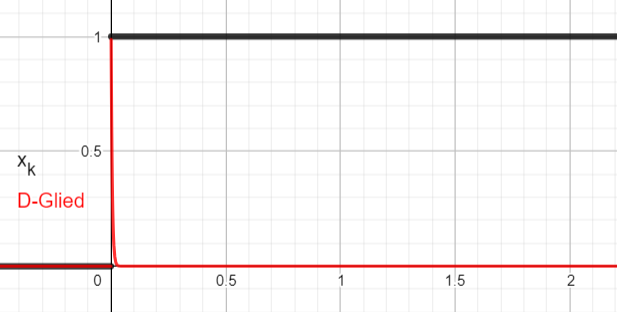
\includegraphics[width=8cm]{Pictures/StepD.png}}
\caption{Sprungantwort eines D-Glieds}
\label{fig:StepD}
\end{center}

\vspace{0.25cm}
\refImgShort{fig:StepD} zeigt die Sprungantwort eines \textit{D-Glieds}. Diese ist ist ein Ausschlag, welcher für den Zeitschritt anhält, in dem sich die ansteigende Flanke des Sprungs befindet.
\end{figure}





\newSec[ControlPID]{PID-Regler}{3}




\begin{equ}[!ht]
\begin{equation}
y_k = y_{k(P)} + y_{k(I)} + y_{k(D)}
\end{equation}
\caption{Übertragungsfunktion des PID-Glieds}
\end{equ}


\begin{figure}[ht!]
\vspace{0.25cm}
\begin{center}
\fbox{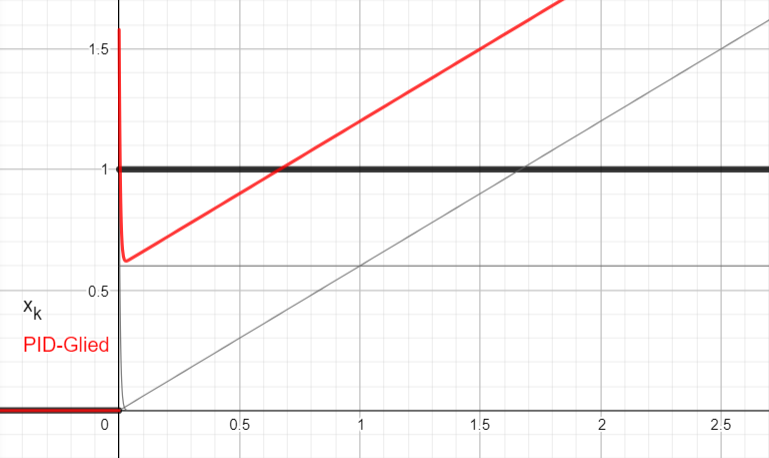
\includegraphics[width=8cm]{Pictures/StepPID.png}}
\caption{Sprungantwort eines PID-Glieds}
\label{fig:StepPID}
\end{center}

\vspace{0.25cm}
\refImgShort{fig:StepPID} zeigt die Sprungantwort eines \textit{PID-Glieds}. Hierbei setzt sich das Signal als Summe des P-, des I- und des D-Glieds zusammen, welche in grau angedeutet sind.
\end{figure}





\newSec[ControlPT]{PT-Glied}{3}

\missing[Dient der Abbildung realer Systeme, welche sich an einen Zustand anpassen müssen. Drehzahlen, Temperaturen etc.]












\begin{equ}[!ht]
\begin{equation}
y_k = k_D * \frac{x_k - x_{k-1}}{\Delta t}
\end{equation}
\caption{Übertragungsfunktion des PT-Glieds}
\end{equ}


\begin{figure}[ht!]
\vspace{0.25cm}
\begin{center}
\fbox{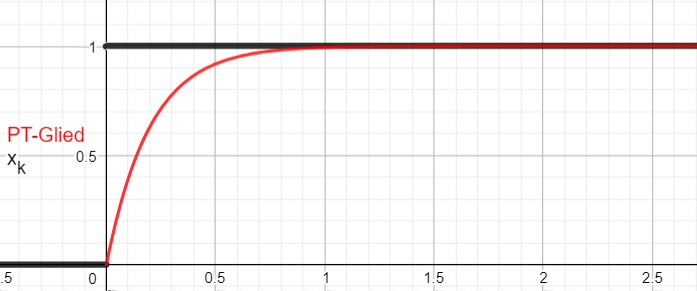
\includegraphics[width=8cm]{Pictures/StepPT.png}}
\caption{Sprungantwort eines PT-Glieds}
\label{fig:StepPT}
\end{center}

\vspace{0.25cm}
\refImgShort{fig:StepPT} zeigt \missing
\end{figure}




\newSec[ControlPT]{Tt-Glied}{3}












